\documentclass[a4paper,sffamily,12pt]{article}

\usepackage[T1]{fontenc}
\usepackage[french]{babel}
\usepackage[utf8]{inputenc}

% Customization des listes
\usepackage{enumitem}
\usepackage{pifont}

% Insertion d'image
\usepackage{graphicx}

% Création de lien
\usepackage[colorlinks,linkcolor=blue]{hyperref}

% Formatage des titres de sections
\usepackage{titlesec}
\titleformat{\section}
  {\normalfont\Large\bfseries\sffamily}{\thesection.}{0.33em}{}[\hrule]
 
 % tableau rectangle 
%\usepackage{slashbox}
%\usepackage{tabularx}

 % En-tête
\usepackage{fancyhdr}
\pagestyle{fancy}
\renewcommand\headrulewidth{1pt}
\fancyhead[L]{Base de données 2}
\fancyhead[R]{$X6I0050$}

% Permet de mettre du texte au dessus du titre
\usepackage{titling}
\renewcommand{\maketitlehooka}{\noindent MAHIER Loïc \hfill groupe 601B \\ JEHANNO Clément \hfill \\ JAMET Félix \hfill \\ PHALAVANDISHVILI  Demetre}

% Titre
\title{\vspace{\fill}\LARGE\bfseries\sffamily Rapport préliminaire de projet\protect\footnote{rapport réalisé sous \LaTeX} \vspace{\fill}}

\begin{document}

	\date{} % Supprime la date
	\maketitle % Affiche le titre

	\thispagestyle{fancy} % Permet de mettre le titre sur la page ''fancy''
	
	\newpage
			
	\renewcommand{\contentsname}{Sommaire}
	\tableofcontents
	
	\newpage
	
	\section{Introduction}
		
		\vspace{0.5cm}
		
		Dans le cadre de ce projet nous devons créer une base de données. Nous avons décidés de modéliser la gestion de cinémas sur une grande échelle. Par exemple nous voulons savoir quels sont les cinémas de France, à qui ils appartiennent (Pathé,UGC, etc.) et ce qu'ils proposent. Comme notre modèle se base sur une certaine réalité voici comment nous avons décomposé la chose, prenons  l'exemple d'un cinéma : \\
		\indent Le cinéma Pathé à Atlantis, dans la ville de Nantes. Tout d'abord on voit que un cinéma est identifié par une adresse et une ville. Ensuite, notre cinéma possède des salles dans lesquelles seront diffusés des films. Chaque film est composé d'une équipe d'acteurs, d'un réalisateur et d'une date de sortie. Il peut être compatible, ou non, à la 3D. \\ 				\indent Nos salle quant à elles, possèdent un certain nombre de places qui sont réparties entre les places "normales" et les places pour les handicapés ainsi que les nouveaux sièges dBox (sièges bougeant en même temps que le film). Si elles sont compatibles, elles ont la possibilité de diffuser en 3D. \\
		\indent Lorsqu'un film est diffusé dans une salle on appelle ça une Séance, notre séance définit le tout c'est à dire "Tel film dans tel cinéma à telle heure". Aujourd'hui si on va au cinéma il est possible de réserver sa séance, autrement dit on réserve pour un film à une horaire précise dans un cinéma donné et le nombre de places que l'on réserve, ainsi que le type de places réservés. 

		\vspace{0.5cm}
								
	\section{Répartitions des tâches}

		\vspace{0.5cm}

		\noindent Voici comment nous nous sommes organisés pour répartir les tâches : \\
		\indent Tout d'abord après les premières semaines de cours nous nous sommes réunis pour décider ensemble d'un sujet. L'idée du cinéma est venue assez naturellement et nous paraissait plutôt bien coller à la réalité pour se pencher dessus.\\
		\indent Ensuite nous avons définis tous les attributs de notre table ensemble, en réfléchissant tous ensemble "on veut faire quoi ? Comment on veut le faire ? Est-ce que un cinéma c'est vraiment comme ça ou pas ? Est-ce que ajouter cet attribut fait du sens ou non" etc. Une fois nos attributs répartits nous avons chacun prit un cinéma (on en a 4) et chaque personne a remplit la partie du tableau qui correspondait à un cinéma. Une fois qu'on a fait ça on a regardé les tuples de notre tableur et on a relevé nos dépendances fonctionnelles.\\
		\indent Ensuite Demetre et Félix ont fait l'algorithme de décomposition et Loïc et Clément on fait l'algorithme de Bernstein. On a mit en commun le résultat des deux algorithmes afin de voir si on avait la même chose ou non, et pourquoi. Pour finir, nous avons testé la normalisation de notre schéma avec l'outil mit à notre disposition en question 5.
						
		\vspace{0.5cm}
		
	\section{Table de base}	
		
		\vspace{0.5cm}
			
		Vous trouverez en annexe la tables (\ref{table_p1}) contenant tous nos attributs ainsi que tous nos tuples. Celle-ci est en quatre partie à cause de sa taille conséquente.
		
		\vspace{0.5cm}						

	\section{Dépendance fonctionnelle}
	
		\vspace{0.5cm}
	
		\noindent- (1) idCine $\rightarrow$ adresse, ville \\
		- (2) adresse, ville $\rightarrow$ franchise, nbsalle \\
		- (3) idCine $\rightarrow$ franchise, nbSalles \\
		- (4) idCine, numSalle $\rightarrow$ SallecompatibleEn3D, nbPlaceStandard, nbPlaceHandicape,nbDbox \\
 		- (5) idFilm $\rightarrow$ nomFilm, dateSortie \\
		- (6) nomFilm, dateSortie $\rightarrow$ public, idReal, duree, compatible3D \\
		- (7) idFilm, role $\rightarrow$  idAct \\
		- (8) idReal $\rightarrow$ nomR, prenomR \\
		- (9) idAct $\rightarrow$ nomA, prenomA \\
		- (10) idClient $\rightarrow$ nomC, prenomC \\
		- (11) idClient, numReservation $\rightarrow$ nbPlaceStandardRes, nbPlaceHandicapeRes, nbPlaceDBoxRes, idSeance \\
		- (12) idSeance, idCine $\rightarrow$ horaire, dateProjection, numSalle, idFilm, diffusionEn3D \\
		
		Avec les dfs ci-dessus, nous obtenons le graphe des dépendances en annexe (\ref{graphe_dependances}). De cela nous déterminons la clé suivante : \{idCine, idClient, numReservation, role\}.
		
	\section{Algo de Bernstein}
	
		\vspace{0.5cm}

		\noindent L'algo de Bernstein se fait en 4 parties :
	
			\begin{enumerate}[label=\ding{228}]
				\item Caclculer la CV(DF) et les clés. Si R est en 3FN, on s'arrête. 
				\item Partitionner CV(DF) e groupe DFi (1 <= i <= k) tels que toutes les df d'un même groupes aient la même partie gauche. 
				\item Construire un schéma <Ri(Ui), DFi> pour chaque groupe DFi, où Ui est l'ensemble des attribut apparaissant dans DFi.
				\item Si aucun des schémas définis ne contient de clé X de R, rajouter un schéma <Rk+1(X), \{\}>.
			\end{enumerate}	
			
		\subsection{Calcul de CV(DF)}

			\vspace{0.5cm}

			\noindent La couverture minimal se fait en trois parties :

			\begin{enumerate}[label=\ding{228}]
				\item Toutes les dépendances doivent être élémentaire ; les décomposer si nécessaire.
				\item Eliminer les attributs superflus du coté gauche de la df.
				\item Eliminer les dfs redondantes.
			\end{enumerate}	
			
			\vspace{0.5cm}
				
			\subsubsection{Pas de 1}

				\vspace{0.5cm}

				\noindent On décompose chacune des dfs : \\

				\noindent- (1) idCine $\rightarrow$ ville \\
				- (1) idCine $\rightarrow$ adresse \\
				- (2) adresse, ville $\rightarrow$ franchise \\
				- (2) adresse, ville $\rightarrow$ nbsalle \\
				- (3) idCine $\rightarrow$ franchise \\
				- (3) idCine $\rightarrow$ nbSalles \\
				- (4) idCine, numSalle $\rightarrow$ SallecompatibleEn3D \\
		 		- (4) idCine, numSalle $\rightarrow$ nbPlaceStandard \\
		 		- (4) idCine, numSalle $\rightarrow$ nbPlaceHandicape \\
		 		- (4) idCine, numSalle $\rightarrow$ nbDbox \\
		 		- (5) idFilm $\rightarrow$ nomFilm \\
		 		- (5) idFilm $\rightarrow$ dateSortie \\				 		
				- (6) nomFilm, dateSortie $\rightarrow$ public \\
				- (6) nomFilm, dateSortie $\rightarrow$ idReal \\
				- (6) nomFilm, dateSortie $\rightarrow$ duree \\
				- (6) nomFilm, dateSortie $\rightarrow$ compatible3D \\
				- (7)idFilm, role $\rightarrow idAct$ \\
				- (8) idReal $\rightarrow$ nomR \\
				- (8) idReal $\rightarrow$ prenomR \\						
				- (9) idAct $\rightarrow$ nomA \\
				- (9) idAct $\rightarrow$ prenomA \\						
				- (10) idClient $\rightarrow$ nomC \\
				- (10) idClient $\rightarrow$ prenomC \\						
				- (11) idClient, numReservation $\rightarrow$ idSeance \\
				- (11) idClient, numReservation $\rightarrow$ nbPlaceStandardRes \\
				- (11) idClient, numReservation $\rightarrow$ nbPlaceHandicapeRes \\
				- (11) idClient, numReservation $\rightarrow$ nbPlaceDBoxRes \\
				- (12) idSeance, idCine $\rightarrow$ horaire \\
				- (12) idSeance, idCine $\rightarrow$ dateProjection \\
				- (12) idSeance, idCine $\rightarrow$ numSalle \\
				- (12) idSeance, idCine $\rightarrow$ idFilm \\
				- (12) idSeance  idCine $\rightarrow$ diffusionEn3D \\
		
				\vspace{0.5cm}
									
			\subsubsection{Pas de 2}

				\vspace{0.5cm}
	
				On prend toutes les dfs qui ont plus d'un attribut à gauche et on calcul leur fermeture. On élimine l'autre attribut si l'attribut de droite de la df apparaît dans le résultat, ou si il apparaît dans le résultat de la fermeture. \\
				
				\noindent - (2) adresse, ville $\rightarrow$ franchise, nbsalle \\
					\\
					\underline{adresse+} \\
					adresse \\
					\underline{ville+} \\
					ville \\
				$\rightarrow$ it's OK \\

				\noindent - (4) idCine, numSalle $\rightarrow$ SallecompatibleEn3D, nbPlaceStandard, nbPlaceHandicape,nbDbox \\
					\\
					\underline{idCine+} \\
					idCine / adresse / ville /franchise / nbSalle \\
					\underline{numSalle+} \\
					numSalle \\
				$\rightarrow$ it's OK \\
				
				\noindent - (6) nomFilm, dateSortie $\rightarrow$ public, idReal, duree, compatible3D \\																						\\
					\underline{nomFilm+} \\
					nomFilm \\
					\underline{dateSotie+} \\
					dateSortie \\
				$\rightarrow$ it's OK \\
			
				\noindent - (7) idFilm, role $\rightarrow$  idAct \\
					\\
					\underline{idFilm+} \\
					idFilm / nomFilm / dateSortie / public / idReal / duree / compatible3D / nomA / prenomA \\
					\underline{role+} \\
					role \\
				$\rightarrow$ it's OK \\
					
				\noindent - (11) idClient, numReservation $\rightarrow$ nbPlaceStandardRes, nbPlaceHandicapeRes, nbPlaceDBoxRes, idSeance \\
					\\
					\underline{idClient+} \\
					idClient / nomC / prenomC \\
					\underline{numReservation+} \\
					numReservation \\	
				$\rightarrow$ it's OK \\					
				
				\noindent - (12) idSeance, idCine $\rightarrow$ horaire, dateProjection, numSalle, idFilm, diffusionEn3D \\												
					\\
					\underline{idSeance+}
					idSeance \\
					\underline{idCine+}
					adresse / ville / franchise / nbSalle \\
				$\rightarrow$ it's OK \\

				\vspace{0.5cm}

			\subsubsection{Pas de 3}		
	
				\vspace{0.5cm}
	
				\noindent Eliminons tout d'abord les dfs qui sont préservées par transitivité : \\
	
					\noindent- (1) idCine $\rightarrow$ adresse, ville \\
					- (2) adresse, ville $\rightarrow$ franchise, nbsalle \\
					- (3) idCine $\rightarrow$ franchise, nbSalles \\
					
				Si l'on prend les dfs 1, 2 et 3, on remarque que l'on peut supprimer la 3 car on peut retrouver celle-ci par transitivité. Reprenons donc nos dfs restantes : \\
					
				\noindent- (1) idCine $\rightarrow$ adresse, ville \\
				- (2) adresse, ville $\rightarrow$ franchise, nbsalle \\
				- (3) idCine, numSalle $\rightarrow$ SallecompatibleEn3D, nbPlaceStandard, nbPlaceHandicape,nbDbox \\
		 		- (4) idFilm $\rightarrow$ nomFilm, dateSortie \\
				- (5) nomFilm, dateSortie $\rightarrow$ public, idReal, duree, compatible3D \\
				- (6) idFilm, role $\rightarrow$  idAct \\
				- (7) idReal $\rightarrow$ nomR, prenomR \\
				- (8) idAct $\rightarrow$ nomA, prenomA \\
				- (9) idClient $\rightarrow$ nomC, prenomC \\
				- (10) idClient, numReservation $\rightarrow$ nbPlaceStandardRes, nbPlaceHandicapeRes, nbPlaceDBoxRes, idSeance \\
				- (11) idSeance, idCine $\rightarrow$ horaire, dateProjection, numSalle, idFilm, diffusionEn3D \\
				
				\noindent A présent, analysons chaque dfs une part une : \\
				
				\noindent - (1) idCine $\rightarrow$ adresse, ville \\
					\\
					\underline{idCine+} \\
					idCine\\									
				$\rightarrow$ it's OK \\		
					
				\noindent - (2) adresse, ville $\rightarrow$ franchise, nbsalle \\
					\\
					\underline{adresse+} \\
					adresse\\
					\underline{ville+} \\
					ville \\									
				$\rightarrow$ it's OK \\
				
				\noindent - (3) idCine, numSalle $\rightarrow$ SallecompatibleEn3D, nbPlaceStandard, nbPlaceHandicape,nbDbox \\
					\\
					\underline{idCine+} \\
					idCIne / adresse / ville / franchise / nbSalle\\
					\underline{numSalle+} \\
					numSalle \\								
				$\rightarrow$ it's OK \\													

				\noindent - (4) idFilm $\rightarrow$ nomFilm, dateSortie \\
					\\
					\underline{idFilm+} \\
					idFilm\\								
				$\rightarrow$ it's OK \\	
				
				\noindent - (5) nomFilm, dateSortie $\rightarrow$ public, idReal, duree, compatible3D \\
					\\
					\underline{nomFilm+} \\
					nomFilm \\
					\underline{dateSortie+} \\
					dateSortie \\									
				$\rightarrow$ it's OK \\	
				
				\noindent - (6) idFilm, role $\rightarrow$  idAct  \\
					\\
					\underline{idFilm+} \\
					idFilm / nomFilm / dateSortie / public / idReal / duree / compatible3D / nomR / prenomR \\
					\underline{role+} \\
					role \\									
				$\rightarrow$ it's OK \\																				
	
				\noindent - (7) idReal $\rightarrow$ nomP, prenomP \\
					\\
					\underline{idReal+} \\
					idReal \\								
				$\rightarrow$ it's OK \\	
				
				\noindent - (8) idAct $\rightarrow$ nomP, prenomP \\
					\\
					\underline{idAct+} \\
					idAct \\									
				$\rightarrow$ it's OK \\	

				\noindent - (9) idClient $\rightarrow$ nomC, prenomC \\
					\\
					\underline{idClient+} \\
					idClient \\									
				$\rightarrow$ it's OK \\		

				\noindent - (10) idClient, numReservation $\rightarrow$ nbPlaceStandardRes, nbPlaceHandicapeRes, nbPlaceDBoxRes, idSeance \\
					\\
					\underline{idClient+} \\
					idClient \ nomC \ prenomC \\
					\underline{numReservation+}
					numReservation \\									
				$\rightarrow$ it's OK \\		

				\noindent - (11) idSeance, idCine $\rightarrow$ horaire, dateProjection, numSalle, idFilm, diffusionEn3D \\
					\\
					\underline{idSeance+} \\
					idSeance \\
					\underline{idCine+}\\
					idCine \\ adresse \ ville \\ franchise \ nbSalle \\							
				$\rightarrow$ it's OK \\							
				\\		
				\noindent Ainsi, hormis la suppression de dfs transitives, nos dfs ne changes pas. \\																
				\\
				On constate que l'on est bien en 1FN, ainsi qu'en 2FN. Cependant nous ne sommes pas en 3eme forme normal. \\
				Ainsi, nous avons des attributs non clés, qui déterminent d'autres attributs non clés. Par exemple, adresse et ville sont deux attributs non clé qui détermine franchise et nbSalle qui sont eux aussi non clés. \\
				
				\vspace{0.5cm}
													
			\subsection{Partitionnement de la CV et construction des schémas} 	
			
				\vspace{0.5cm}
			
				\noindent R1 = \{idCine, adresse, ville\} \\  DF1 = \{idCine $\rightarrow$ adresse, ville\} \\
				\\
				R2 = \{idCine, franchise, nbSalle\} \\ DF2 = \{adresse, ville $\rightarrow$ franchise, nbSalle\} \\
				\\
				R3 = \{idCine, numSalle, salleCompatibleEn3D, nbPlaceStanard, nbPlaceHandicapes, nbDbox\} \\ DF3 = \{idCine, numSalle, $\rightarrow$ salleCompatibleEn3D, nbPlaceStanard, nbPlaceHandicapes, nbDbox\} \\
				\\
				R4 = \{idFilm, nomFilm, dateSortie\} \\ DF4 = \{idFilm $\rightarrow$ nomFilm, dateSortie\} \\
				\\
				R5 = \{idFilm\} \\ DF5 = \{nomFilm, dateSortie $\rightarrow$ public, idReal, duree, compatible3D\} \\	
				\\							
				R6 = \{idFilm, role, idAct\} \\ DF6 = \{idFilm, role $\rightarrow$  idAct\} \\
				\\
				R7 = \{idReal, nomR, prenomR\} \\ DF7 = \{idReal $\rightarrow$ nomR, prenomR\} \\
				\\
				R8 = \{idAct, nomA, prenomA\} \\ DF8 = \{idAct $\rightarrow$ nomA, prenomA\} \\
				\\
				R9 = \{idClient, nomC, prenomC\} \\ DF9 = \{idClient $\rightarrow$ nomC, prenomC\} \\ 
				\\
				R10 = \{idClient, numReservation, nbPlaceStandardRes, nbPlaceHandicapesRes, nbPlaceDBoxRes, idSeance\} \\ DF10 = \{idClient, numReservation $\rightarrow$  nbPlaceStandardRes, nbPlaceHandicapesRes, nbPlaceDBoxRes, idSeance\} \\
				\\
				R11 = \{idSeance, idCine, horaire, dateProjection, numSalle, idFilm, diffusionEn3D\} \\ DF11 = \{idSeance, idCine $\rightarrow$ horaire, dateProjection, numSalle, idFilm, diffusionEn3D\} \\
				
				\vspace{0.5cm}
								
			\subsection{Ajout d'un schéma} 	

				\vspace{0.5cm}
											
				\noindent R12 = \{idCine, idClient, numReservation, role\} \\ DF12 = \{\} \\

				\vspace{0.5cm}

		\section{Algo de décomposition}

			\vspace{0.5cm}
			
			Nous avons pris tous nos attributs puis on a suivi l'algorithme de décomposition c'est à dire que en fonction de nos attributs et de nos dépendances fonctionnelles on a pris une dépendance, on a fait une relation en fonction de cette dépendance puis on a retiré nos attributs non clés au reste de la relation originale. Ensuite on a recommencé jusqu'à arriver à une partie qui ne contient que des clés et plus de df.\\
			\indent On a commencé par les df qui n'avaient que un attribut à gauche puis on a finit par celles qui avaient plusieurs attributs à gauche.
		
			



			\vspace{0.5cm}

		\section{Schéma de nos tables}
		
		Pour le diagramme nous nous sommes basés sur le résultat de l'algorithme de décomposition qui nous a fournit des tables équivalentes aux 11 relations R1..R11. Cependant nous avons fusionnés deux fois deux tables : la table R1 et R21 car ça nous paraît plus logique d'avoir pour chaque adresse, ville, franchise et nbsalles un seul idCine qui en fait détermine un unique cinéma.\\
		\indent Cette table devient donc la table Cinéma ce qui donne plus de sens à notre modèle. Nous avons aussi fusionné R51 et R61 pour en faire une seule et même table Film, pour les mêmes raisons.\\
		\indent Pour finir on a renommé toutes les autres tables pour leur donner un nom qui nous parle plus : R31 est devenue Réalisateur, R41 est devenue Acteur, R71 est devenue Client, R81 est devenue Salle, R91 est devenue Casting, R101 est devenue Seance, 111 est devenue Réservation.

				\begin{figure}[!h]		
					\centering
					{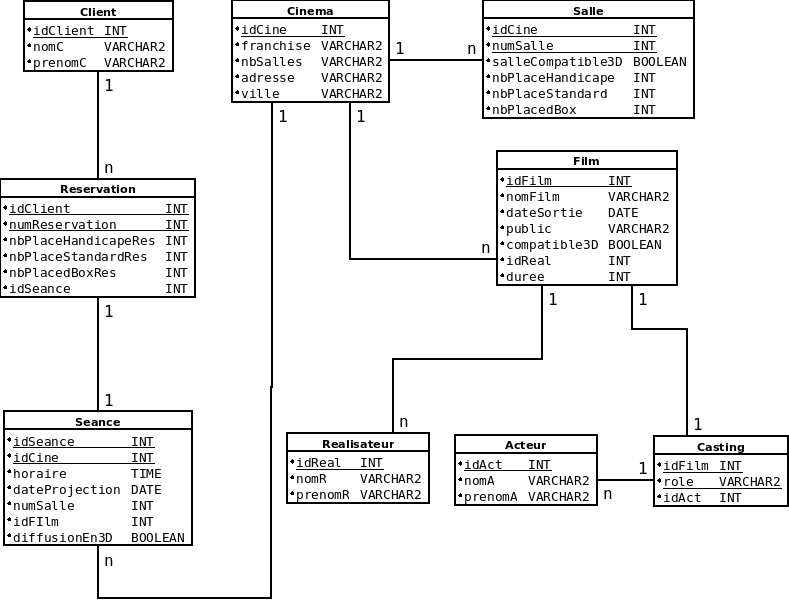
\includegraphics[height=11cm]{picture/DiagrammeUML.png}}
					\caption{DiagrammeUML de nos tables}
					\label{UML}	
				\end{figure}		

		\section{Conclusion}

			\vspace{0.5cm}
			
			
			

			\newpage

			\section{Annexe}
							
				\begin{figure}[!h]		
					\centering
					\rotatebox{90}{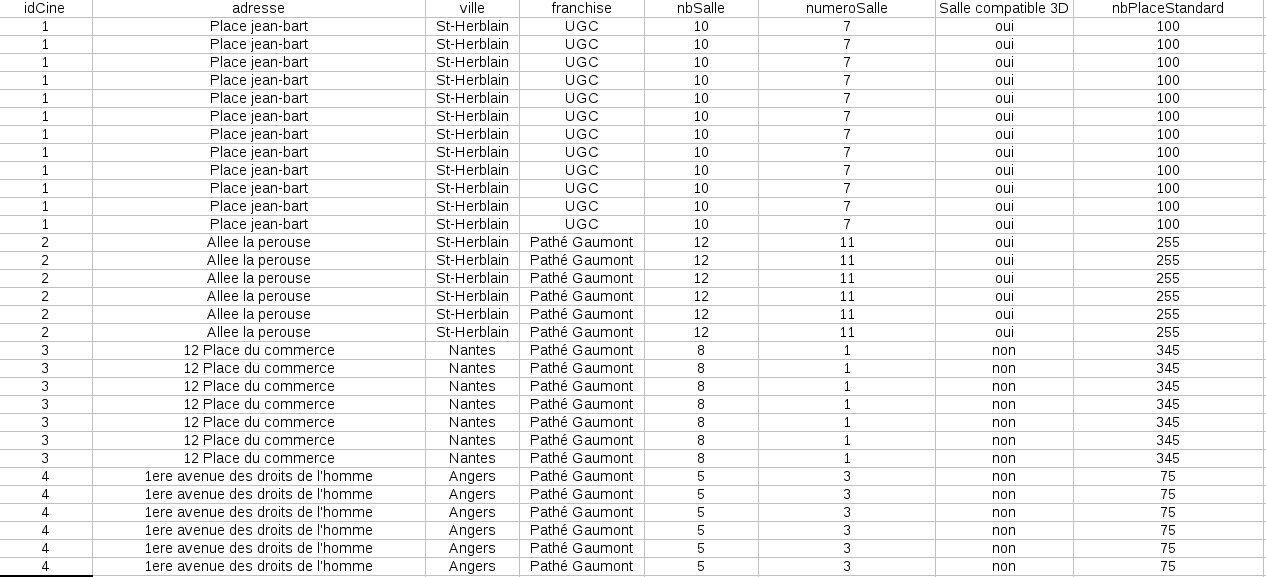
\includegraphics[height=8cm]{picture/table_p1_rogne.png}}
					\caption{Première partie de notre table contenant tous les attributs et quelques tuples}
					\label{table_p1}	
				\end{figure}			

				\begin{figure}[!h]
					\centering						
					\rotatebox{90}{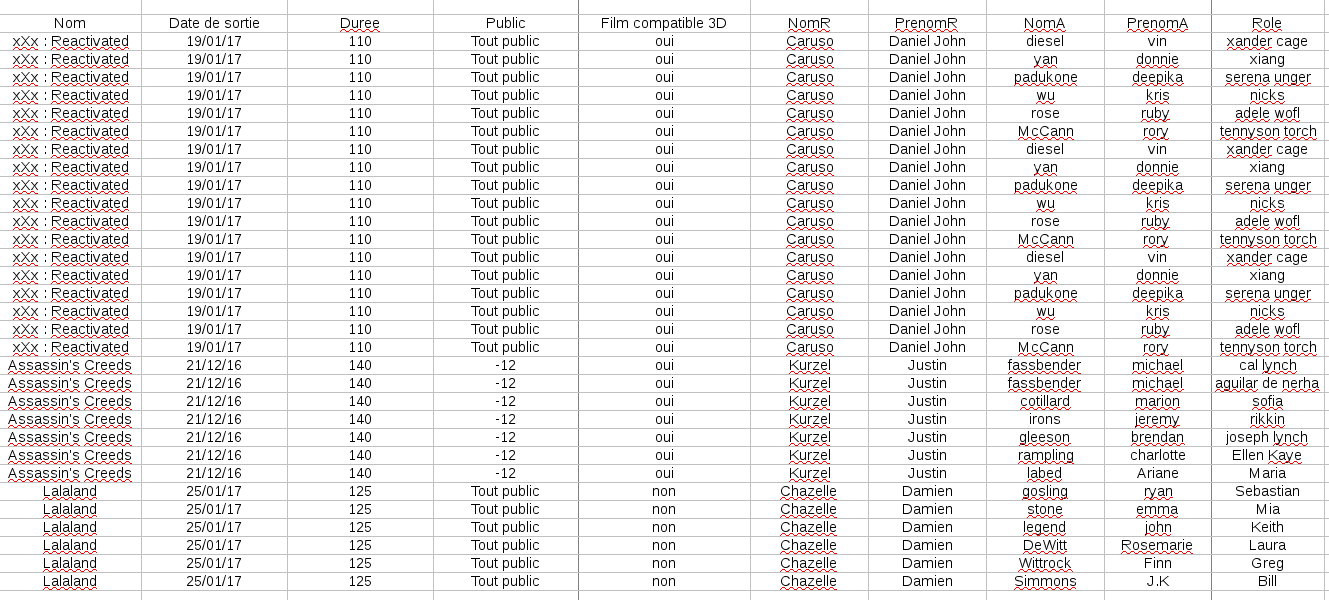
\includegraphics[height=8cm]{picture/table_p2_rogne.png}}
					\caption{Deuxième partie de notre table contenant tous les attributs et quelques tuples}
					\label{table_p2}	
				\end{figure}			

				\begin{figure}[!h]
					\centering						
					\rotatebox{90}{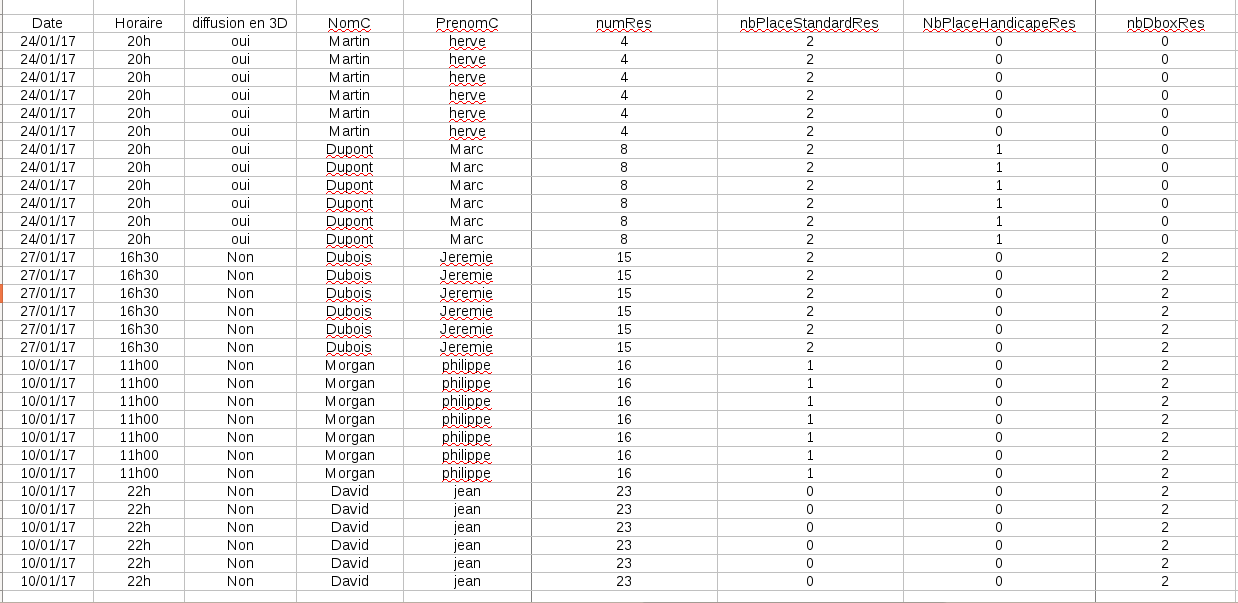
\includegraphics[height=9cm]{picture/table_p3_rogne.png}}
					\caption{Troisième partie de notre table contenant tous les attributs et quelques tuples}
					\label{table_p3}	
				\end{figure}	

				\begin{figure}[!h]
					\centering						
					\rotatebox{90}{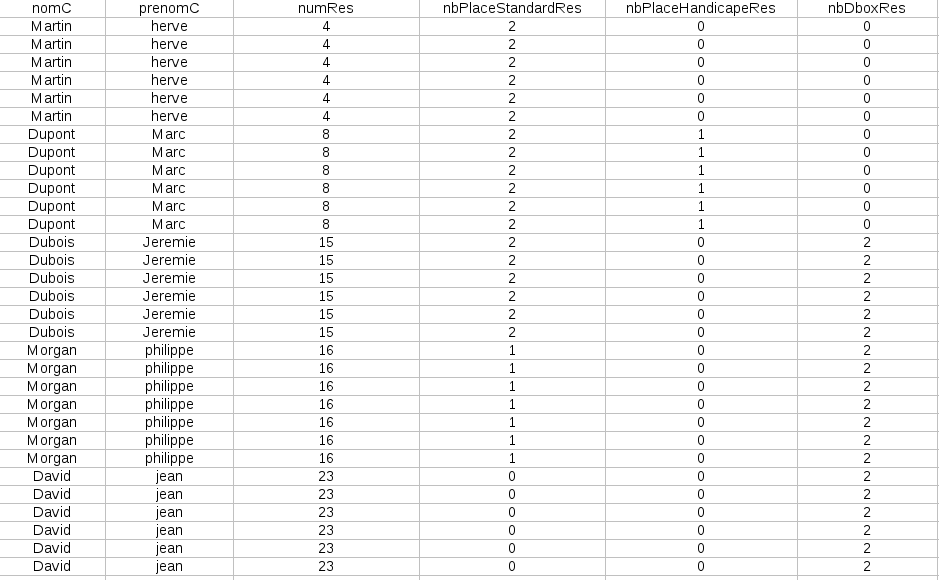
\includegraphics[height=10cm]{picture/table_p4_rogne.png}}
					\caption{Quatrième partie de notre table contenant tous les attributs et quelques tuples}
					\label{table_p4}	
				\end{figure}
				
				\begin{figure}[!h]
					\centering						
					\rotatebox{90}{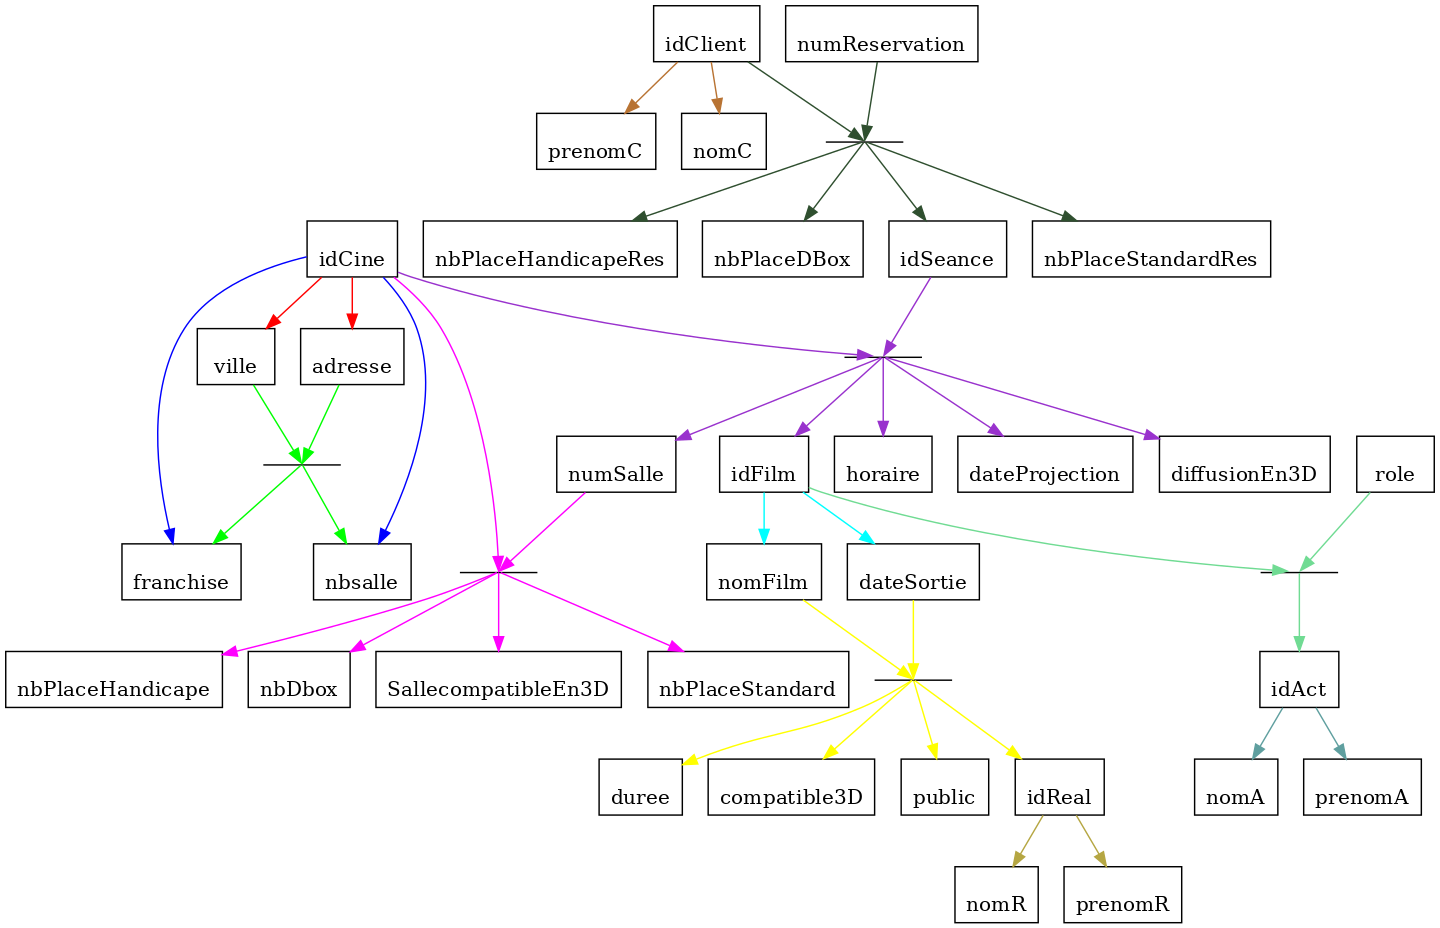
\includegraphics[height=8cm]{picture/graphe_dependances.png}}
					\caption{Graphes des dépendances}
					\label{graphe_dependances}	
				\end{figure}	
					
\end{document}